\begin{scanpage}{0028}{11}
The direction $\phi=\pi-\phi_0$ corresponds to the ray reflected in a specular fashion from the first face (we will consider as the first face that face from which the angles are calculated), and the direction $\phi=2\alpha-\pi-\phi_0$ corresponds to the ray reflected specularly from the second face (Figure 5 and 6). The functions $e^{-ikr\cos\psi}$ describe plane waves of unit amplitude: $e^{-ikr\cos(\phi-\phi_0)}$ describes the incident wave, $e^{-ikr\cos(\phi+\phi_0)}$ describes the wave reflected from the first face, and $e^{-ikr\cos(2\alpha-\phi-\phi_0)}$ --- the wave reflected from the second face.
\begin{center}\begin{minipage}[t]{.48\linewidth}\vspace{0pt}\centering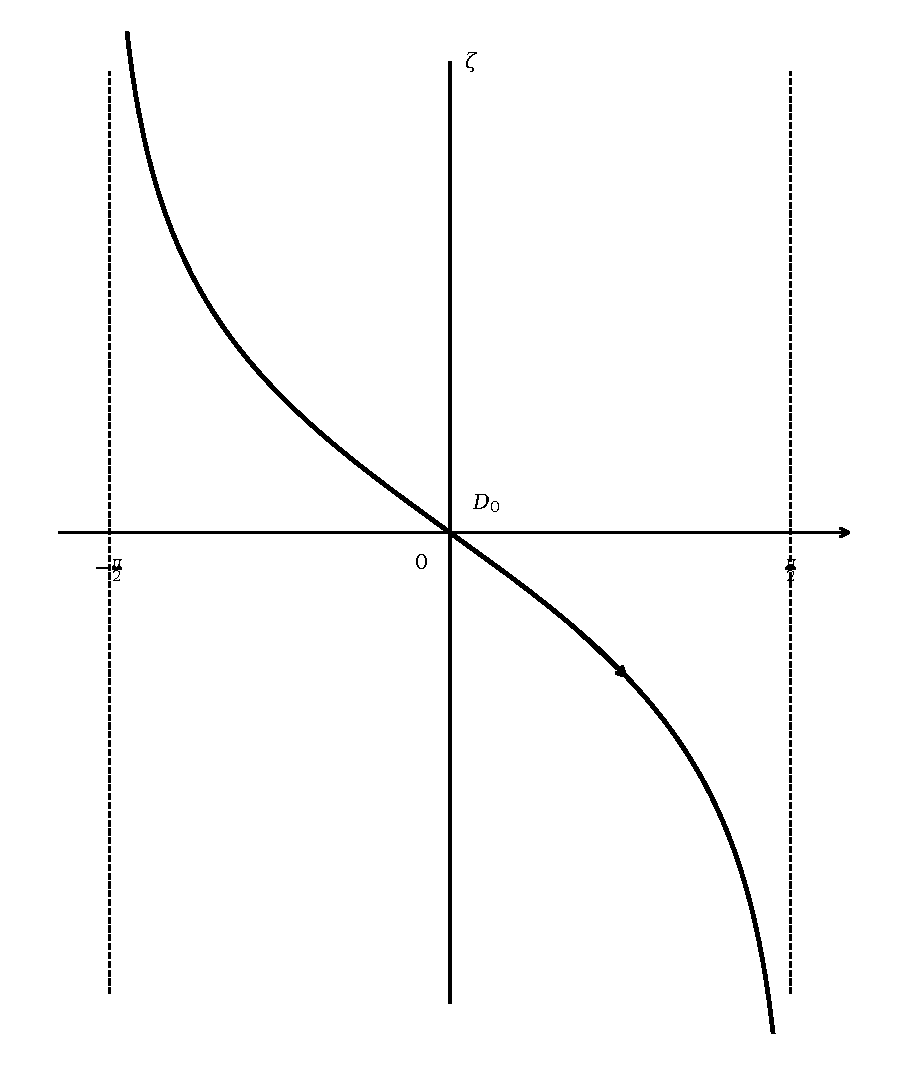
\includegraphics[width=.8\linewidth,height=4cm,keepaspectratio]{images/recreated/a-0028-fig4.pdf}\par Figure 4. The integration contour in Equation (1.30).\end{minipage}\hfill\begin{minipage}[t]{.48\linewidth}\vspace{0pt}\centering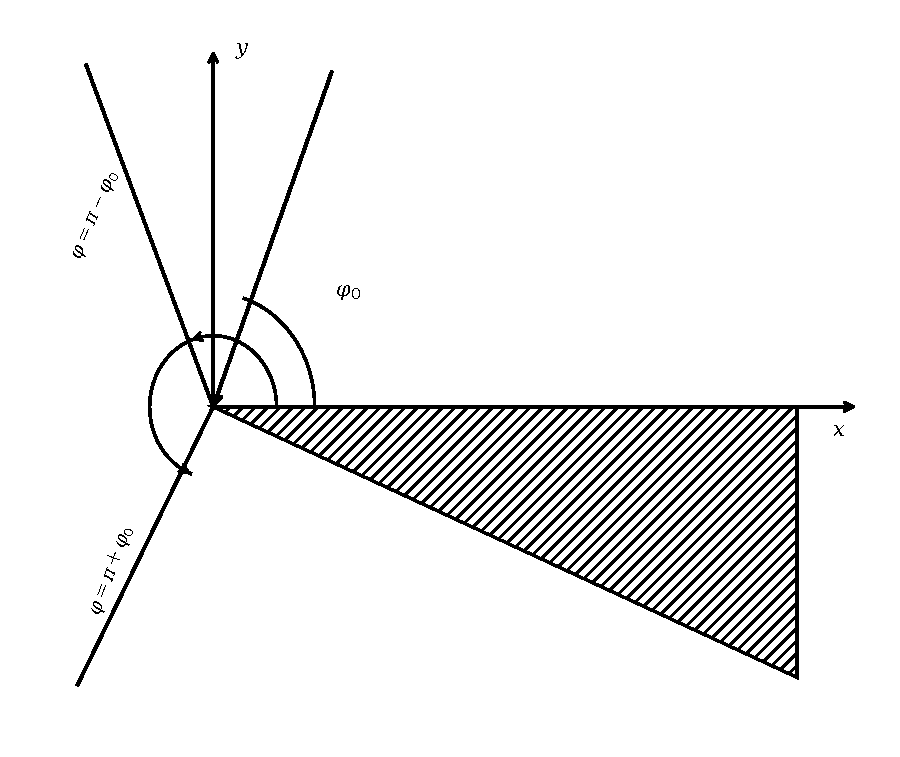
\includegraphics[width=.8\linewidth,height=3cm,keepaspectratio]{images/recreated/a-0028-fig5.pdf}\par Figure 5. Diffraction of a plane wave by a wedge. The plane wave irradiates only one face of the wedge. $\phi_0$ is the angle of incidence. The line $\phi=\pi-\phi_0$ is the boundary of the reflected plane wave, and the line $\phi=\pi+\phi_0$ is the boundary of the shadow.\end{minipage}\par\medskip
\begin{minipage}{.48\linewidth}\centering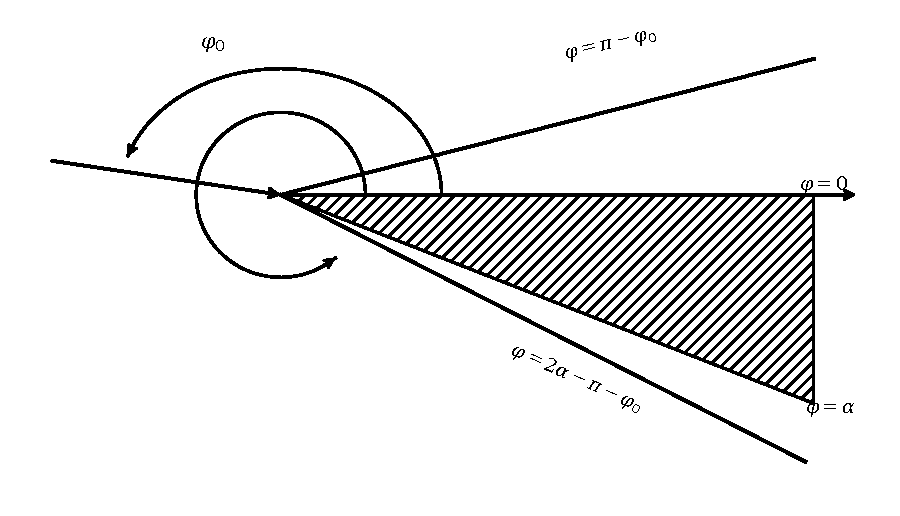
\includegraphics[width=.95\linewidth]{images/recreated/a-0028-fig6.pdf}\end{minipage}\hfill\begin{minipage}{.48\linewidth}Figure 6. Diffraction by a wedge. The plane wave irradiates both faces. The line $\phi=2\alpha-\pi-\phi_0$ is the boundary of the plane wave reflected from the second face $(\phi=\alpha)$.\end{minipage}\end{center}
\end{scanpage}
